% ============================================================================
% Pedagogical solutions: Discrete Mathematics - Practice 1 (Set Theory).
% Problems 2, 7, 11, 16, 20, 54(3,11), 58, 60.
% English, pdflatex. Source kept ASCII-clean (no em-dashes, no curly quotes).
% Compile: pdflatex twice.
% ============================================================================
\documentclass[11pt,a4paper]{article}

% ---- Encoding & fonts ----
\usepackage[utf8]{inputenc}
\usepackage[T1]{fontenc}
\usepackage{lmodern}

% ---- Math ----
\usepackage{amsmath,amssymb,amsthm}
\usepackage{mathtools}

% ---- Layout ----
\usepackage[margin=2.3cm]{geometry}
\usepackage{enumitem}
\usepackage{booktabs}
\usepackage{array}

% ---- Visuals ----
\usepackage{xcolor}
\usepackage[most]{tcolorbox}
\usepackage{tikz}
\usetikzlibrary{arrows.meta,positioning,calc,fit,backgrounds,shapes.misc,shapes.geometric,decorations.pathreplacing}
\usepackage{pgfplots}
\pgfplotsset{compat=1.18}
\usepackage{hyperref}
\hypersetup{colorlinks=true,linkcolor=blue!55!black,urlcolor=blue!55!black}

% ---- Palette (Armenian flag colours; use for 3+ series plots) ----
\definecolor{armRed}{HTML}{D90012}
\definecolor{armBlue}{HTML}{0033A0}
\definecolor{armOrange}{HTML}{F2A800}
\definecolor{ink}{HTML}{22303C}

\setlength{\parindent}{0pt}
\setlength{\parskip}{5pt}

% ---- Math shortcuts ----
\newcommand{\Z}{\mathbb{Z}}
\newcommand{\R}{\mathbb{R}}
\newcommand{\N}{\mathbb{N}}
\newcommand{\setdiff}{\setminus}
\DeclareMathOperator{\sd}{}            % placeholder, unused
\newcommand{\symd}{\triangle}          % symmetric difference (written div in the source)

% ---- Boxes ----
\newtcolorbox{problembox}[1][]{enhanced, breakable, sharp corners=south,
  colback=armOrange!10, colframe=armOrange!75!black, boxrule=0.8pt, arc=2mm,
  fonttitle=\bfseries\color{white}, coltitle=white,
  attach boxed title to top left={xshift=4mm,yshift=-2.4mm},
  boxed title style={colback=armOrange!85!black, arc=1mm},
  title={Problem #1}}

\newtcolorbox{ideabox}{enhanced, breakable,
  colback=armBlue!6, colframe=armBlue!70!black, boxrule=0.8pt, arc=2mm,
  fonttitle=\bfseries\color{white}, coltitle=white,
  attach boxed title to top left={xshift=4mm,yshift=-2.4mm},
  boxed title style={colback=armBlue!75!black, arc=1mm},
  title={The idea}}

\newtcolorbox{methodbox}{enhanced, breakable,
  colback=gray!8, colframe=gray!55!black, boxrule=0.7pt, arc=2mm,
  fonttitle=\bfseries, title={$\bigstar$\ Method to remember}}

\newtcolorbox{answerbox}{enhanced, sharp corners=south,
  colback=green!8, colframe=green!50!black, boxrule=1pt, arc=2mm, left=4mm,right=4mm}
\newcommand{\answer}[1]{\begin{answerbox}\centering\textbf{Answer:}\quad #1\end{answerbox}}

% ---- Title ----
\title{\vspace{-1.2cm}\textbf{Discrete Mathematics - Practical 1}\\[2pt]
\large Set Theory: worked solutions\\[2pt]
\normalsize\itshape with the reasoning spelled out, step by step}
\author{}
\date{}

\begin{document}
\maketitle
\vspace{-1.0cm}

\begin{center}\small\itshape Covers the assigned subset of Practical 1: problems 2, 7, 11, 16, 20, 54 (parts 3 and 11), 58, 60.\end{center}

\section*{Warm-up}

This sheet is mostly about \emph{proving} set statements, not computing numbers. Three kinds of
task appear. (1) \textbf{Membership puzzles} (problems 2, 7, 11): keep a clear head about the
difference between an element $x$ and the one-element set $\{x\}$ that contains it; $\in$ and
$\subseteq$ are different relations. (2) \textbf{Set identities} (16, 20, 54, 60): the universal
tool is \emph{element-chasing} - to prove $X=Y$, show that an arbitrary element lies in $X$ if and
only if it lies in $Y$, by rewriting the defining condition step by step. (3) A small
\textbf{construction / structural} argument (58).

Notation used here: $\overline{A}$ is the complement of $A$ (everything in the universe $U$ that
is not in $A$); $A\setminus B$ is set difference (in the source sheet it is written $A-B$);
$A\symd B$ is the \emph{symmetric difference} (written $\div$ in the source), defined by
$A\symd B=(A\setminus B)\cup(B\setminus A)$; and $\subset$ means \emph{strict} inclusion
($A\subseteq B$ and $A\neq B$), while $\subseteq$ allows equality.

The single most useful habit on this sheet: when stuck, drop down to the level of one element.
Almost every line below is just \textquotedbl{}what does it mean for a fixed $x$ to belong here?\textquotedbl{}

% ============================================================================
% PROBLEM 2
% ============================================================================
\section*{Problem 2 - Which membership statements are true?}

\begin{problembox}[2]
Decide which of the following are true.
\begin{enumerate}[label=\textbf{2.\arabic*},leftmargin=2.2cm]
\item $\varnothing \in \{\varnothing,\ \{\varnothing\}\}$
\item $\{\varnothing\} \in \{\{\varnothing\}\}$
\item $\varnothing \in \{\{\varnothing\}\}$
\end{enumerate}
\end{problembox}

\begin{ideabox}
$x\in S$ is true exactly when $x$ is \emph{literally one of the items listed inside the braces of}
$S$ - nothing more. So read each set as a list and ask: is the thing on the left one of the entries
on the right? The only trap is that the entries can themselves be sets, and you must not confuse
$\varnothing$ (the empty set, $0$ elements) with $\{\varnothing\}$ (a box containing the empty set,
$1$ element). They are different objects, so $\varnothing\neq\{\varnothing\}$. Treat
$\varnothing$ and $\{\varnothing\}$ as two distinct \textquotedbl{}names\textquotedbl{} and just
scan the list.
\end{ideabox}

\textbf{Step 1 - List the entries of each right-hand set.}
\begin{itemize}[leftmargin=1.4cm]
\item $\{\varnothing,\ \{\varnothing\}\}$ has \emph{two} entries: $\varnothing$ and $\{\varnothing\}$.
\item $\{\{\varnothing\}\}$ has \emph{one} entry: $\{\varnothing\}$.
\end{itemize}

\textbf{Step 2 - Check each claim against the list.}
\begin{itemize}[leftmargin=1.4cm]
\item \textbf{2.1} $\varnothing \in \{\varnothing,\{\varnothing\}\}$: is $\varnothing$ one of the
two entries? Yes, it is the first one. \textbf{True.}
\item \textbf{2.2} $\{\varnothing\} \in \{\{\varnothing\}\}$: is $\{\varnothing\}$ the single
entry? Yes, the entry is exactly $\{\varnothing\}$. \textbf{True.}
\item \textbf{2.3} $\varnothing \in \{\{\varnothing\}\}$: is $\varnothing$ the single entry? The
only entry is $\{\varnothing\}$, and $\varnothing\neq\{\varnothing\}$ (zero elements versus one).
So no. \textbf{False.}
\end{itemize}

\textbf{Always check.} A quick sanity test that 2.3 is genuinely false: $\{\{\varnothing\}\}$ has
exactly one element. If both $\varnothing$ and $\{\varnothing\}$ belonged to it, it would have two
distinct elements. It does not, so at most one of them is in it - and 2.2 already pinned that one
down as $\{\varnothing\}$. \checkmark

\textbf{The three objects as nested boxes} (a box is a set; what sits loose inside it are its
elements). Reading them side by side shows why they are all different:

\begin{center}
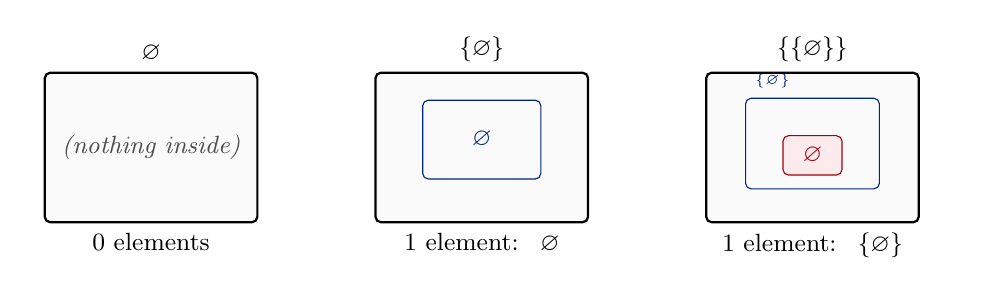
\begin{tikzpicture}[font=\small,
  outer/.style={draw, thick, rounded corners=2pt, minimum width=2.7cm, minimum height=1.9cm},
  mid/.style={draw, armBlue!75!black, rounded corners=2pt, minimum width=1.5cm, minimum height=1.0cm},
  inn/.style={draw, armRed!75!black, rounded corners=2pt, minimum width=0.75cm, minimum height=0.5cm, fill=armRed!8}]
% --- object 1: empty set ---
\node[outer, fill=gray!4] (o1) at (0,0) {};
\node[anchor=south] at (o1.north) {$\varnothing$};
\node[gray!60!black] at (o1) {\itshape (nothing inside)};
\node[anchor=north, text width=2.9cm, align=center] at (o1.south) {$0$ elements};
% --- object 2: {empty set} ---
\node[outer, fill=gray!4] (o2) at (4.2,0) {};
\node[anchor=south] at (o2.north) {$\{\varnothing\}$};
\node[mid] (o2m) at (4.2,0.1) {$\varnothing$};
\node[anchor=north, text width=3.4cm, align=center] at (o2.south) {$1$ element: \ $\varnothing$};
% --- object 3: {{empty set}} ---
\node[outer, fill=gray!4] (o3) at (8.4,0) {};
\node[anchor=south] at (o3.north) {$\{\{\varnothing\}\}$};
\node[mid, minimum width=1.7cm, minimum height=1.15cm] (o3m) at (8.4,0.05) {};
\node[inn] (o3i) at (8.4,-0.1) {$\varnothing$};
\node[anchor=south west, font=\tiny, armBlue!75!black] at (o3m.north west) {$\{\varnothing\}$};
\node[anchor=north, text width=3.6cm, align=center] at (o3.south) {$1$ element: \ $\{\varnothing\}$};
\end{tikzpicture}
\end{center}

\answer{2.1 True, \quad 2.2 True, \quad 2.3 False.}

\begin{methodbox}
\textbf{Transferable technique:} $x\in S$ asks only \textquotedbl{}is $x$ an item in the
top-level list of $S$?\textquotedbl{}. Do not look inside the items. And always keep
$x$ separate from $\{x\}$: wrapping something in braces makes a new, different object with one
element.
\end{methodbox}

% ============================================================================
% PROBLEM 7
% ============================================================================
\section*{Problem 7 - $\in$ is not transitive}

\begin{problembox}[7]
Give sets $A,B,C$ with $A\in B$, $B\in C$, but $A\notin C$.
\end{problembox}

\begin{ideabox}
For relations like $\le$ or $\subseteq$, chaining works: $a\le b\le c$ forces $a\le c$. The point
of this exercise is that \emph{membership $\in$ does not chain}. $A\in B$ says $A$ sits one level
down inside $B$; $B\in C$ says $B$ sits one level down inside $C$, so $A$ is now \emph{two} levels
down inside $C$ - which is a completely different statement from \textquotedbl{}$A$ is an element
of $C$\textquotedbl{}. The cleanest way to feel this is to build a tower where each set is wrapped
once more in braces. The classic tower is $\varnothing,\ \{\varnothing\},\ \{\{\varnothing\}\}$.
\end{ideabox}

\textbf{Step 1 - Choose the tower.}
Let
$$A=\varnothing,\qquad B=\{\varnothing\},\qquad C=\{\{\varnothing\}\}.$$

\textbf{Step 2 - Verify the two memberships.}
\begin{itemize}[leftmargin=1.4cm]
\item $A\in B$: is $\varnothing$ an entry of $\{\varnothing\}$? Yes. \checkmark
\item $B\in C$: is $\{\varnothing\}$ an entry of $\{\{\varnothing\}\}$? Yes, it is the only entry. \checkmark
\end{itemize}

\textbf{Step 3 - Verify the non-membership.}
$C=\{\{\varnothing\}\}$ has a single entry, $\{\varnothing\}$. Is $A=\varnothing$ that entry? No,
$\varnothing\neq\{\varnothing\}$. So $A\notin C$. \checkmark

\answer{$A=\varnothing,\quad B=\{\varnothing\},\quad C=\{\{\varnothing\}\}$. \quad This witnesses that $\in$ is not transitive.}

\medskip
\textbf{Picture of the nesting} (each box is one level; $A$ is buried two levels deep inside $C$,
so it is not a direct entry of $C$):

\begin{center}
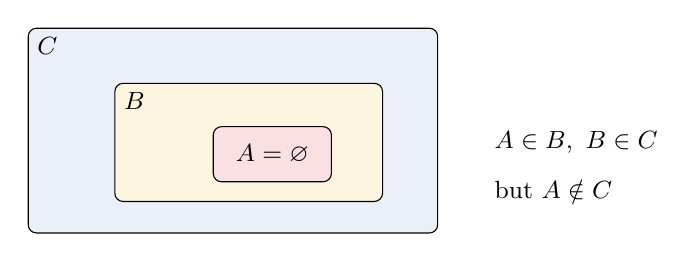
\begin{tikzpicture}[font=\small,
  lvl/.style={draw, rounded corners=3pt, inner sep=6pt}]
% C
\node[lvl, fill=armBlue!8, minimum width=5.2cm, minimum height=2.6cm] (C) at (0,0) {};
\node[anchor=north west] at (C.north west) {\textbf{$C$}};
% B inside C
\node[lvl, fill=armOrange!12, minimum width=3.4cm, minimum height=1.5cm] (B) at (0.2,-0.15) {};
\node[anchor=north west] at (B.north west) {\textbf{$B$}};
% A inside B
\node[lvl, fill=armRed!12, minimum width=1.5cm, minimum height=0.7cm] (A) at (0.5,-0.3) {$A=\varnothing$};
\node[anchor=west] at (3.2,-0.15) {$A\in B,\ B\in C$};
\node[anchor=west] at (3.2,-0.75) {but $A\notin C$};
\end{tikzpicture}
\end{center}

% ============================================================================
% PROBLEM 11
% ============================================================================
\section*{Problem 11 - A mixed inclusion / membership chain}

\begin{problembox}[11]
Give sets $A,B,C,D,E$ with $A\subset B$, $B\in C$, $C\subset D$, $D\subset E$, where every
$\subset$ is strict.
\end{problembox}

\begin{ideabox}
The puzzle mixes two different relations in one chain, and the only awkward link is the middle
one, $B\in C$: here $B$ must appear as a whole \emph{element} of $C$, not as a subset. So engineer
$C$ so that one of its listed entries is exactly the set $B$. Everything else is routine: for a
strict inclusion $X\subset Y$, just take $Y$ to be $X$ with one extra element thrown in. Build
$A\subset B$ first, then make $C$ a set that \emph{contains $B$ as an item}, then keep adding one
element to climb $C\subset D\subset E$.
\end{ideabox}

\textbf{Step 1 - The strict pair $A\subset B$.}
Take $A=\{1\}$ and $B=\{1,2\}$. Then $A\subseteq B$ and $A\neq B$, so $A\subset B$ (strict). \checkmark

\textbf{Step 2 - Put $B$ as an element of $C$.}
We need $B=\{1,2\}$ to be an \emph{entry} of $C$. Take
$$C=\{\,\{1,2\},\,3\,\}.$$
Its two entries are the set $\{1,2\}$ and the number $3$. Since $\{1,2\}=B$ is one of them,
$B\in C$. \checkmark
(Note this is membership, not inclusion: $B$ is an item inside $C$.)

\textbf{Step 3 - Climb with strict inclusions.}
Add one fresh element at each step:
$$D=\{\,\{1,2\},\,3,\,4\,\},\qquad E=\{\,\{1,2\},\,3,\,4,\,5\,\}.$$
Then $C\subset D$ (all of $C$ is in $D$, and $4\in D\setminus C$) and $D\subset E$ (and
$5\in E\setminus D$). Both strict. \checkmark

\textbf{The chain, with $\in$ and $\subset$ drawn differently.} Nesting (one oval/box inside
another) means $\subseteq$; a set sitting as one \emph{loose item} in a list means $\in$. The
single $\in$ link is $B$ appearing as one element of $C$:

\begin{center}
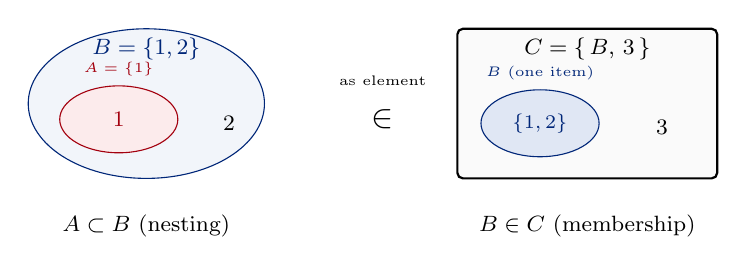
\begin{tikzpicture}[font=\footnotesize]
% --- A subset B : nested ovals ---
\node[draw, armBlue!75!black, ellipse, minimum width=3.0cm, minimum height=1.9cm, fill=armBlue!5] (Bset) at (0,0) {};
\node[anchor=north] at (Bset.north) {\color{armBlue!75!black}$B=\{1,2\}$};
\node[draw, armRed!75!black, ellipse, minimum width=1.5cm, minimum height=0.85cm, fill=armRed!8] (Aset) at (-0.35,-0.2) {$1$};
\node[anchor=south, font=\tiny, armRed!75!black] at (Aset.north) {$A=\{1\}$};
\node at (1.05,-0.25) {$2$};
\node at (0,-1.55) {$A\subset B$ (nesting)};
% --- arrow ---
\node at (3.0,-0.2) {\large $\in$};
\node[anchor=south, font=\tiny] at (3.0,0.1) {as element};
% --- C box containing B as one element, plus 3 ---
\node[draw, thick, rounded corners=2pt, minimum width=3.3cm, minimum height=1.9cm, fill=gray!4] (Cset) at (5.6,0) {};
\node[anchor=north] at (Cset.north) {$C=\{\,B,\,3\,\}$};
\node[draw, armBlue!75!black, ellipse, minimum width=1.5cm, minimum height=0.85cm, fill=armBlue!12] (Bin) at (5.0,-0.25) {\scriptsize $\{1,2\}$};
\node[anchor=south, font=\tiny, armBlue!75!black] at (Bin.north) {$B$ (one item)};
\node at (6.55,-0.3) {$3$};
\node at (5.6,-1.55) {$B\in C$ (membership)};
\end{tikzpicture}

\medskip
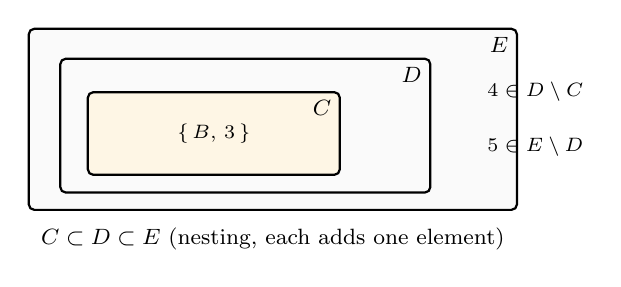
\begin{tikzpicture}[font=\footnotesize,
  bx/.style={draw, thick, rounded corners=2pt, fill=gray!4}]
% nested boxes C subset D subset E
\node[bx, minimum width=6.2cm, minimum height=2.3cm] (E) at (0,0) {};
\node[anchor=north east] at (E.north east) {$E$};
\node[bx, minimum width=4.7cm, minimum height=1.7cm] (D) at (-0.35,-0.08) {};
\node[anchor=north east] at (D.north east) {$D$};
\node[bx, fill=armOrange!10, minimum width=3.2cm, minimum height=1.05cm] (C) at (-0.75,-0.18) {\scriptsize $\{\,B,\,3\,\}$};
\node[anchor=north east] at (C.north east) {$C$};
\node[anchor=west] at (2.6,0.35) {\scriptsize $4\in D\setminus C$};
\node[anchor=west] at (2.6,-0.35) {\scriptsize $5\in E\setminus D$};
\node[anchor=north] at (0,-1.25) {$C\subset D\subset E$ (nesting, each adds one element)};
\end{tikzpicture}
\end{center}

\answer{$A=\{1\},\ B=\{1,2\},\ C=\{\{1,2\},3\},\ D=\{\{1,2\},3,4\},\ E=\{\{1,2\},3,4,5\}$.}

\begin{methodbox}
\textbf{Transferable technique:} to force \textquotedbl{}$B\in C$\textquotedbl{}, list $B$ itself
as one of the elements of $C$ (do not merge $B$'s elements into $C$ - that would give
$B\subseteq C$ instead). To force a \emph{strict} inclusion $X\subset Y$, take $Y=X\cup\{\text{one
new element}\}$.
\end{methodbox}

% ============================================================================
% PROBLEM 16
% ============================================================================
\section*{Problem 16 - Describe the derived sets}

\begin{problembox}[16]
Let the universe be $U=\Z$, and
\begin{gather*}
A=\{x\in\Z:\exists y\in\Z^{+},\ x=2y\},\qquad
  B=\{x\in\Z:\exists y\in\Z^{+},\ x=2y-1\},\\
  C=\{x\in\Z:x<10\}.
\end{gather*}
Describe the sets $\overline{A}$, \ $\overline{A\cup B}$, \ $\overline{C}$, \ $A\setminus C$, \
$C\setminus(A\cup B)$.
\end{problembox}

\begin{ideabox}
First translate each defining condition into plain words, then everything is bookkeeping on the
integer line. Because $y$ ranges over the \emph{positive} integers $\Z^{+}=\{1,2,3,\dots\}$:
\begin{itemize}[leftmargin=1.2cm,topsep=2pt]
\item $x=2y$ with $y\ge 1$ gives $A=\{2,4,6,\dots\}$, the \textbf{positive even} integers.
\item $x=2y-1$ with $y\ge 1$ gives $B=\{1,3,5,\dots\}$, the \textbf{positive odd} integers.
\item $C=\{x:x<10\}=\{\dots,7,8,9\}$, all integers \textbf{below} $10$.
\end{itemize}
The one observation that makes the rest fall out: every positive integer is either even or odd, so
$A\cup B=\Z^{+}=\{1,2,3,\dots\}$. A complement $\overline{X}$ is \textquotedbl{}$U$ minus
$X$\textquotedbl{} ($U=\Z$), and a difference is \textquotedbl{}keep, then remove\textquotedbl{}.
Reading these off a number line makes the answers obvious.
\end{ideabox}

\textbf{Step 1 - The two basic unions.}
$A\cup B$ is all positive evens together with all positive odds, i.e. \emph{all positive
integers}: $A\cup B=\Z^{+}=\{1,2,3,\dots\}$.

\textbf{Step 2 - Read off each set.}
\begin{itemize}[leftmargin=1.4cm]
\item $\overline{A}=\Z\setminus\{2,4,6,\dots\}$: every integer that is \emph{not} a positive even,
namely all integers $x\le 0$ together with all positive odd numbers
($\{\dots,-2,-1,0\}\cup\{1,3,5,\dots\}$).
\item $\overline{A\cup B}=\Z\setminus\Z^{+}=\{0,-1,-2,\dots\}=\{x\in\Z:x\le 0\}$ (the non-positive
integers: zero and the negatives).
\item $\overline{C}=\Z\setminus\{x<10\}=\{x\in\Z:x\ge 10\}=\{10,11,12,\dots\}$.
\item $A\setminus C$: positive evens that are \emph{not} below $10$, i.e. positive evens
$\ge 10$: $\{10,12,14,\dots\}$.
\item $C\setminus(A\cup B)$: integers below $10$ with all positive integers removed, leaving the
non-positive ones: $\{0,-1,-2,\dots\}=\{x\in\Z:x\le 0\}$. This is the \emph{same} set as
$\overline{A\cup B}$ (every $x\le 0$ is below $10$, so removing $\Z^{+}$ from $\Z$ or from
$\{x<10\}$ leaves the same thing).
\end{itemize}

\textbf{Always check (number line, window $-3$ to $12$).}
The illustration below tracks $A$ (positive evens) and $B$ (positive odds). One can verify by eye:
$A\setminus C$ starts at $10$; $\overline{C}$ is everything from $10$ up; and both
$\overline{A\cup B}$ and $C\setminus(A\cup B)$ are exactly the points $\le 0$.
A brute-force enumeration over $-20\le x\le 20$ confirms all five descriptions and the equality
$C\setminus(A\cup B)=\overline{A\cup B}$. \checkmark

\begin{center}
\resizebox{\textwidth}{!}{%
\begin{tikzpicture}[font=\footnotesize,>=Stealth]
\def\xlo{-3}\def\xhi{12}
% axis
\draw[<->] (\xlo-0.6,0) -- (\xhi+0.8,0) node[right]{$\Z$};
\foreach \x in {-3,...,12}{
  \draw (\x,0.08) -- (\x,-0.08);
  \node[below] at (\x,-0.1) {\tiny \x};
}
% threshold at 10 (C is x<10)
\draw[armOrange!80!black, dashed] (9.5,-0.5) -- (9.5,1.7);
\node[armOrange!70!black, anchor=south] at (9.5,1.7) {\tiny $x<10\ |\ x\ge 10$};
% positive evens A (red squares) up to 12
\foreach \x in {2,4,6,8,10,12}{
  \fill[armRed] (\x,0.55) circle (2.6pt);
}
\node[armRed, anchor=west] at (\xhi+0.2,0.55) {};
\node[armRed] at (\xlo-0.9,0.55) {\tiny $A$};
% positive odds B (blue) up to 11
\foreach \x in {1,3,5,7,9,11}{
  \draw[armBlue, fill=white, line width=0.8pt] (\x,1.05) circle (2.6pt);
}
\node[armBlue] at (\xlo-0.9,1.05) {\tiny $B$};
% mark non-positive region (<=0) for (AuB)bar
\draw[decorate, decoration={brace, amplitude=4pt}, gray!60!black]
  (\xlo-0.55,-0.55) -- (0,-0.55);
\node[gray!60!black, anchor=north] at (-1.5,-0.62) {\tiny $\overline{A\cup B}=C\setminus(A\cup B)=\{x\le 0\}$};
% legend
\node[anchor=west] at (\xlo-0.6,1.7) {\tiny \textcolor{armRed}{$\bullet$} positive evens $A$\quad \textcolor{armBlue}{$\circ$} positive odds $B$};
\end{tikzpicture}%
}
\end{center}

\answer{$\overline{A}=\{x\le 0\}\cup\{1,3,5,\dots\}$;\quad
$\overline{A\cup B}=\{x\le 0\}=\{0,-1,-2,\dots\}$;\quad
$\overline{C}=\{10,11,12,\dots\}$;\quad
$A\setminus C=\{10,12,14,\dots\}$;\quad
$C\setminus(A\cup B)=\{x\le 0\}\ (=\overline{A\cup B})$.}

\begin{methodbox}
\textbf{Transferable technique:} decode each set-builder into one plain sentence first
(\textquotedbl{}positive evens\textquotedbl{}, \textquotedbl{}integers below $10$\textquotedbl{}),
spot the structural fact that simplifies everything ($A\cup B=\Z^{+}$), then read complements as
\textquotedbl{}$U$ minus the set\textquotedbl{} and differences as \textquotedbl{}keep then
remove\textquotedbl{}. A number line turns it into something you can just look at.
\end{methodbox}

% ============================================================================
% PROBLEM 20
% ============================================================================
\section*{Problem 20 - Three families of equivalent conditions}

\begin{problembox}[20]
Let $A,B$ be arbitrary subsets of a universe $U$. Prove that in each row, all the listed
conditions are equivalent.
\begin{enumerate}[label=\textbf{Row \arabic*:},leftmargin=2cm]
\item $A\subseteq B\ \Longleftrightarrow\ \overline{B}\subseteq\overline{A}\ \Longleftrightarrow\
A\cup B=B\ \Longleftrightarrow\ A\cap B=A$.
\item $A\cap B=\varnothing\ \Longleftrightarrow\ A\subseteq\overline{B}\ \Longleftrightarrow\
B\subseteq\overline{A}$.
\item $A\cup B=U\ \Longleftrightarrow\ \overline{A}\subseteq B\ \Longleftrightarrow\
\overline{B}\subseteq A$.
\end{enumerate}
\end{problembox}

\begin{ideabox}
\textquotedbl{}These four conditions are equivalent\textquotedbl{} means: any one of them implies
every other. Proving all $4\cdot 3=12$ implications separately is wasteful. The efficient trick is
a \textbf{cycle of implications}: prove
$$P_1\Rightarrow P_2\Rightarrow P_3\Rightarrow P_4\Rightarrow P_1.$$
Once the cycle closes, you can get from any condition to any other by walking around the loop, so
all four are equivalent. We show Row 1 in full this way. For Rows 2 and 3 the three conditions in a
row are, on the level of a single element $x$, three rephrasings of one implication (for Row 2 it
is \textquotedbl{}$x\in A\Rightarrow x\notin B$\textquotedbl{}; for Row 3 it is
\textquotedbl{}$x\notin A\Rightarrow x\in B$\textquotedbl{}), so a short element argument settles
each row at once.
\end{ideabox}

\textbf{Row 1 - the cycle
$A\subseteq B\Rightarrow A\cup B=B\Rightarrow A\cap B=A\Rightarrow \overline{B}\subseteq\overline{A}\Rightarrow A\subseteq B$.}

\begin{enumerate}[label=(\alph*),leftmargin=1.2cm]
\item $A\subseteq B\Rightarrow A\cup B=B$.\\
Always $B\subseteq A\cup B$. Conversely, if $x\in A\cup B$ then $x\in A$ or $x\in B$; in the first
case $A\subseteq B$ gives $x\in B$, in the second $x\in B$ already. So $A\cup B\subseteq B$. Both
inclusions give $A\cup B=B$.
\item $A\cup B=B\Rightarrow A\cap B=A$.\\
From $A\cup B=B$ and $A\subseteq A\cup B$ we get $A\subseteq B$. Then for any $x\in A$ we also have
$x\in B$, so $x\in A\cap B$; hence $A\subseteq A\cap B$. The reverse $A\cap B\subseteq A$ is always
true. So $A\cap B=A$.
\item $A\cap B=A\Rightarrow \overline{B}\subseteq\overline{A}$.\\
$A\cap B=A$ says $A\subseteq B$ (every element of $A$ is in $A\cap B$, hence in $B$). Now take
$x\in\overline{B}$, i.e. $x\notin B$. If $x$ were in $A$, then $x\in B$ by $A\subseteq B$ - a
contradiction. So $x\notin A$, i.e. $x\in\overline{A}$. Thus $\overline{B}\subseteq\overline{A}$.
\item $\overline{B}\subseteq\overline{A}\Rightarrow A\subseteq B$.\\
This is the contrapositive of (c). Take $x\in A$. Then $x\notin\overline{A}$; since
$\overline{B}\subseteq\overline{A}$, also $x\notin\overline{B}$, i.e. $x\in B$. Thus
$A\subseteq B$.
\end{enumerate}
The cycle is closed, so all four conditions of Row 1 are equivalent. $\blacksquare$

\textbf{Row 2 - $A\cap B=\varnothing\Leftrightarrow A\subseteq\overline{B}\Leftrightarrow B\subseteq\overline{A}$.}\\
Read each condition for a single element $x$:
$$A\cap B=\varnothing
\ \Longleftrightarrow\ \text{no }x\text{ lies in both}
\ \Longleftrightarrow\ \bigl(x\in A\Rightarrow x\notin B\bigr)
\ \Longleftrightarrow\ \bigl(x\in A\Rightarrow x\in\overline{B}\bigr)
\ \Longleftrightarrow\ A\subseteq\overline{B}.$$
The middle implication \textquotedbl{}$x\in A\Rightarrow x\notin B$\textquotedbl{} is symmetric in
$A,B$ (it equals \textquotedbl{}$x\in B\Rightarrow x\notin A$\textquotedbl{}, i.e.
$x\in B\Rightarrow x\in\overline{A}$, i.e. $B\subseteq\overline{A}$). So all three are equivalent.
$\blacksquare$

\textbf{Row 3 - $A\cup B=U\Leftrightarrow \overline{A}\subseteq B\Leftrightarrow \overline{B}\subseteq A$.}\\
Again at the element level:
$$A\cup B=U
\ \Longleftrightarrow\ \text{every }x\text{ is in }A\text{ or }B
\ \Longleftrightarrow\ \bigl(x\notin A\Rightarrow x\in B\bigr)
\ \Longleftrightarrow\ \overline{A}\subseteq B.$$
The implication \textquotedbl{}$x\notin A\Rightarrow x\in B$\textquotedbl{} is the contrapositive
of \textquotedbl{}$x\notin B\Rightarrow x\in A$\textquotedbl{}, which is $\overline{B}\subseteq A$.
So all three are equivalent. $\blacksquare$

\textbf{Always check.} An exhaustive computer check over all pairs of subsets $A,B$ of a $5$-element
universe confirms that within each row the conditions are simultaneously true or simultaneously
false (no pair separates them). \checkmark

\textbf{Seeing the equivalences.} Each condition is a picture. When the four Row 1 panels all
describe the \emph{same} arrangement (A nested inside B), the equivalence is visible at a glance;
likewise the single panel for each of Rows 2 and 3. (Shaded $=$ the set named under the panel;
the outer rectangle is the universe $U$.)

\begin{center}
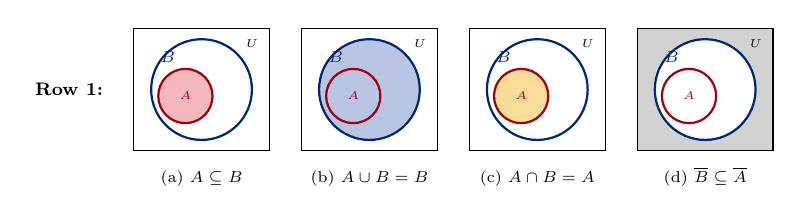
\begin{tikzpicture}[font=\scriptsize, scale=0.82, every node/.style={transform shape}]
% rectangle = U, A nested inside B (A small, B large); shade the named set per panel
% ---------- Row 1 label ----------
\node[anchor=east, font=\footnotesize\bfseries] at (-1.4,0) {Row 1:};
% ---------- (a) A subseteq B : shade A ----------
\begin{scope}[shift={(0,0)}]
  \fill[armRed!28] (-0.25,-0.1) circle (0.42);
  \draw[armBlue!75!black, thick] (0.0,0) circle (0.78);
  \draw[armRed!75!black, thick] (-0.25,-0.1) circle (0.42);
  \node[armBlue!75!black] at (-0.52,0.5) {$B$};
  \node[armRed!75!black, font=\tiny] at (-0.25,-0.1) {$A$};
  \draw (-1.05,-0.95) rectangle (1.05,0.95);
  \node[anchor=north east, font=\tiny] at (1.0,0.9) {$U$};
  \node[anchor=south, align=center] at (0,-1.62) {(a) $A\subseteq B$};
\end{scope}
% ---------- (b) AuB = B : shade B ----------
\begin{scope}[shift={(2.6,0)}]
  \fill[armBlue!28] (0,0) circle (0.78);
  \draw[armBlue!75!black, thick] (0,0) circle (0.78);
  \draw[armRed!75!black, thick] (-0.25,-0.1) circle (0.42);
  \node[armBlue!75!black] at (-0.52,0.5) {$B$};
  \node[armRed!75!black, font=\tiny] at (-0.25,-0.1) {$A$};
  \draw (-1.05,-0.95) rectangle (1.05,0.95);
  \node[anchor=north east, font=\tiny] at (1.0,0.9) {$U$};
  \node[anchor=south, align=center] at (0,-1.62) {(b) $A\cup B=B$};
\end{scope}
% ---------- (c) AnB = A : shade A ----------
\begin{scope}[shift={(5.2,0)}]
  \fill[armOrange!40] (-0.25,-0.1) circle (0.42);
  \draw[armBlue!75!black, thick] (0,0) circle (0.78);
  \draw[armRed!75!black, thick] (-0.25,-0.1) circle (0.42);
  \node[armBlue!75!black] at (-0.52,0.5) {$B$};
  \node[armRed!75!black, font=\tiny] at (-0.25,-0.1) {$A$};
  \draw (-1.05,-0.95) rectangle (1.05,0.95);
  \node[anchor=north east, font=\tiny] at (1.0,0.9) {$U$};
  \node[anchor=south, align=center] at (0,-1.62) {(c) $A\cap B=A$};
\end{scope}
% ---------- (d) Bbar subseteq Abar : shade complement of B ----------
\begin{scope}[shift={(7.8,0)}]
  \fill[gray!35] (-1.05,-0.95) rectangle (1.05,0.95);
  \fill[white] (0,0) circle (0.78);
  \draw[armBlue!75!black, thick] (0,0) circle (0.78);
  \draw[armRed!75!black, thick] (-0.25,-0.1) circle (0.42);
  \node[armBlue!75!black] at (-0.52,0.5) {$B$};
  \node[armRed!75!black, font=\tiny] at (-0.25,-0.1) {$A$};
  \draw (-1.05,-0.95) rectangle (1.05,0.95);
  \node[anchor=north east, font=\tiny] at (1.0,0.9) {$U$};
  \node[anchor=south, align=center] at (0,-1.62) {(d) $\overline{B}\subseteq\overline{A}$};
\end{scope}
\end{tikzpicture}

\medskip
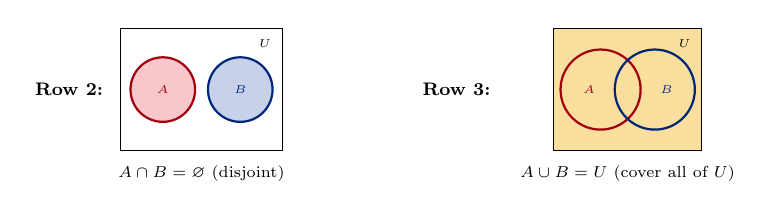
\begin{tikzpicture}[font=\scriptsize, scale=0.82, every node/.style={transform shape}]
% ---------- Row 2: A n B = empty : disjoint ----------
\node[anchor=east, font=\footnotesize\bfseries] at (-1.4,0) {Row 2:};
\begin{scope}[shift={(0,0)}]
  \fill[armRed!22] (-0.6,0) circle (0.5);
  \fill[armBlue!22] (0.6,0) circle (0.5);
  \draw[armRed!75!black, thick] (-0.6,0) circle (0.5);
  \draw[armBlue!75!black, thick] (0.6,0) circle (0.5);
  \node[armRed!75!black, font=\tiny] at (-0.6,0) {$A$};
  \node[armBlue!75!black, font=\tiny] at (0.6,0) {$B$};
  \draw (-1.25,-0.95) rectangle (1.25,0.95);
  \node[anchor=north east, font=\tiny] at (1.2,0.9) {$U$};
  \node[anchor=south, align=center] at (0,-1.55) {$A\cap B=\varnothing$ (disjoint)};
\end{scope}
% ---------- Row 3: A u B = U : circles cover all ----------
\node[anchor=east, font=\footnotesize\bfseries] at (4.6,0) {Row 3:};
\begin{scope}[shift={(6.6,0)}]
  \fill[armOrange!38] (-1.15,-0.95) rectangle (1.15,0.95);
  \draw[armRed!75!black, thick] (-0.42,0) circle (0.62);
  \draw[armBlue!75!black, thick] (0.42,0) circle (0.62);
  \node[armRed!75!black, font=\tiny] at (-0.6,0) {$A$};
  \node[armBlue!75!black, font=\tiny] at (0.6,0) {$B$};
  \draw (-1.15,-0.95) rectangle (1.15,0.95);
  \node[anchor=north east, font=\tiny] at (1.1,0.9) {$U$};
  \node[anchor=south, align=center] at (0,-1.55) {$A\cup B=U$ (cover all of $U$)};
\end{scope}
\end{tikzpicture}
\end{center}

\answer{All conditions in each row are equivalent; Row 1 is proved by the implication cycle
$A\subseteq B\Rightarrow A\cup B=B\Rightarrow A\cap B=A\Rightarrow \overline{B}\subseteq\overline{A}\Rightarrow A\subseteq B$, and Rows 2--3 by a single element-level implication read three ways.}

\begin{methodbox}
\textbf{Transferable technique:} to show several conditions are equivalent, do not prove every
pairwise implication - prove a single \emph{cycle} $P_1\Rightarrow P_2\Rightarrow\cdots\Rightarrow
P_n\Rightarrow P_1$. Equivalences involving complements are often cleanest via the
\emph{contrapositive} ($\overline{B}\subseteq\overline{A}$ is just $A\subseteq B$ read backwards).
\end{methodbox}

% ============================================================================
% PROBLEM 54
% ============================================================================
\section*{Problem 54 - Two set identities (parts 3 and 11)}

\begin{problembox}[54]
Prove the identities.
\begin{enumerate}[label=\textbf{(\arabic*)},leftmargin=1.4cm]
\item[\textbf{(3)}] $(A\cup B)\setminus C=(A\setminus C)\cup(B\setminus C)$.
\item[\textbf{(11)}] $A\cap(B\symd C)=(A\cap B)\symd(A\cap C)$, \quad where
$X\symd Y=(X\setminus Y)\cup(Y\setminus X)$ \ (symmetric difference, written $\div$ in the source).
\end{enumerate}
\end{problembox}

\begin{ideabox}
The one reliable engine for set identities is \textbf{element-chasing}: to prove $X=Y$, take a
fixed $x$ and show $x\in X\Leftrightarrow x\in Y$ by unfolding the definitions
($\cup\to$\textquotedbl{}or\textquotedbl{}, $\cap\to$\textquotedbl{}and\textquotedbl{},
$\setminus\to$\textquotedbl{}and not\textquotedbl{}) and rearranging by simple logic. Part (3) is a
clean distributive law and falls straight out. Part (11) mixes in symmetric difference; the key
realization is that $x\in X\symd Y$ means \textquotedbl{}$x$ is in \emph{exactly one} of
$X,Y$\textquotedbl{} - a parity statement. After conditioning on whether $x\in A$, the
\textquotedbl{}exactly one\textquotedbl{} bookkeeping lines up on both sides.
\end{ideabox}

\textbf{Part (3) - distributing $\setminus C$ over $\cup$.}
Element-chase:
\begin{align*}
x\in(A\cup B)\setminus C
&\iff (x\in A\ \text{or}\ x\in B)\ \text{and}\ x\notin C\\
&\iff (x\in A\ \text{and}\ x\notin C)\ \text{or}\ (x\in B\ \text{and}\ x\notin C)
   &&\text{[\textquotedbl{}and\textquotedbl{} distributes over \textquotedbl{}or\textquotedbl{}]}\\
&\iff x\in(A\setminus C)\ \text{or}\ x\in(B\setminus C)\\
&\iff x\in(A\setminus C)\cup(B\setminus C).
\end{align*}
Since this holds for every $x$, the two sets are equal. $\blacksquare$

\textbf{Part (11) - intersection distributes over symmetric difference.}
Recall $x\in X\symd Y\iff x$ belongs to \emph{exactly one} of $X,Y$. Fix an arbitrary $x$ and split
on membership in $A$.

\emph{Case $x\notin A$.} Then $x\notin A\cap(B\symd C)$ (left side). Also $x\notin A\cap B$ and
$x\notin A\cap C$, so $x$ is in \emph{neither} $A\cap B$ nor $A\cap C$, hence
$x\notin(A\cap B)\symd(A\cap C)$ (right side). Both sides exclude $x$. \checkmark

\emph{Case $x\in A$.} Then $x\in A\cap B\iff x\in B$ and $x\in A\cap C\iff x\in C$. Therefore
\begin{align*}
x\in(A\cap B)\symd(A\cap C)
&\iff x\ \text{is in exactly one of}\ A\cap B,\ A\cap C\\
&\iff x\ \text{is in exactly one of}\ B,\ C &&\text{[}x\in A\text{, so }A\cap\ \text{is automatic]}\\
&\iff x\in B\symd C\\
&\iff x\in A\cap(B\symd C) &&\text{[because }x\in A\text{].}
\end{align*}
So on $\{x\in A\}$ the two sides agree as well. As both cases match, the sets are equal.
$\blacksquare$

\textbf{Always check.} Exhaustive enumeration over all triples $A,B,C$ of subsets of a $4$-element
ground set finds \emph{zero} disagreements for both identities. A Venn check for (3): the region
\textquotedbl{}in $A$ or $B$, outside $C$\textquotedbl{} is precisely the two crescents
\textquotedbl{}in $A$, outside $C$\textquotedbl{} and \textquotedbl{}in $B$, outside
$C$\textquotedbl{} taken together. \checkmark

\begin{center}
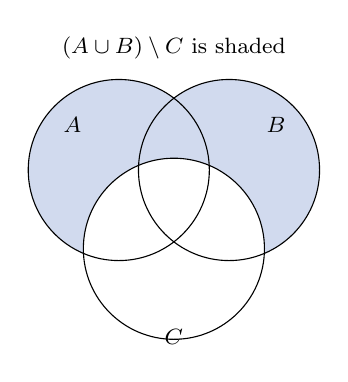
\begin{tikzpicture}[font=\footnotesize]
% Venn for (3): A, B, C three circles, shade (AuB)\C
\def\rA{1.15}
\begin{scope}
% clip to (A u B) and outside C, shade
\begin{scope}
  \clip (-0.7,0) circle (\rA) (0.7,0) circle (\rA);
  \fill[armBlue!18] (-3,-2) rectangle (3,2);
\end{scope}
% punch out C
\begin{scope}
  \clip (-0.7,0) circle (\rA) (0.7,0) circle (\rA);
  \fill[white] (0,-1.0) circle (\rA);
\end{scope}
\draw (-0.7,0) circle (\rA) node[above left=0.5cm] {$A$};
\draw (0.7,0) circle (\rA) node[above right=0.5cm] {$B$};
\draw (0,-1.0) circle (\rA) node[below=0.9cm] {$C$};
\node at (0,1.55) {$(A\cup B)\setminus C$ is shaded};
\end{scope}
\end{tikzpicture}
\end{center}

\textbf{Part (11) as a picture.} Both sides shade the \emph{same} region: the two slivers of $A$
that lie in exactly one of $B,C$. Three circles $A$ (top), $B$ (lower left), $C$ (lower right):

\begin{center}
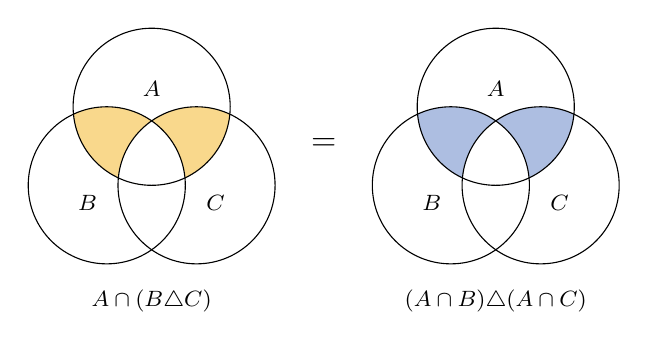
\begin{tikzpicture}[font=\footnotesize, scale=0.95]
% coordinates and radius shared by both panels
\def\r{1.05}
% positions: A top, B lower-left, C lower-right
% ---------------- LEFT panel: A cap (B sym-diff C) ----------------
\begin{scope}[shift={(0,0)}]
  % shade A and (in B xor C): clip to A, then to (B or C), then punch out (B and C)
  \begin{scope}
    \clip (0,0.55) circle (\r);                       % inside A
    \begin{scope}
      \clip (-0.6,-0.5) circle (\r) (0.6,-0.5) circle (\r);  % inside (B or C)
      \fill[armOrange!45] (-2,-2.2) rectangle (2,1.9);
    \end{scope}
    % punch out B cap C (the part in both B and C)
    \begin{scope}
      \clip (-0.6,-0.5) circle (\r);
      \fill[white] (0.6,-0.5) circle (\r);
    \end{scope}
  \end{scope}
  \draw (0,0.55) circle (\r) node[above] {$A$};
  \draw (-0.6,-0.5) circle (\r) node[below left] {$B$};
  \draw (0.6,-0.5) circle (\r) node[below right] {$C$};
  \node at (0,-2.05) {$A\cap(B\symd C)$};
\end{scope}
% ---------------- RIGHT panel: (A cap B) sym-diff (A cap C) ----------------
\begin{scope}[shift={(4.6,0)}]
  % (A n B) xor (A n C): in A, and in exactly one of B,C  -> identical region
  \begin{scope}
    \clip (0,0.55) circle (\r);                       % inside A (forced by both A n B and A n C)
    \begin{scope}
      \clip (-0.6,-0.5) circle (\r) (0.6,-0.5) circle (\r);  % inside (B or C)
      \fill[armBlue!32] (-2,-2.2) rectangle (2,1.9);
    \end{scope}
    \begin{scope}
      \clip (-0.6,-0.5) circle (\r);
      \fill[white] (0.6,-0.5) circle (\r);            % punch out B cap C
    \end{scope}
  \end{scope}
  \draw (0,0.55) circle (\r) node[above] {$A$};
  \draw (-0.6,-0.5) circle (\r) node[below left] {$B$};
  \draw (0.6,-0.5) circle (\r) node[below right] {$C$};
  \node at (0,-2.05) {$(A\cap B)\symd(A\cap C)$};
\end{scope}
\node at (2.3,0.05) {\large $=$};
\end{tikzpicture}
\end{center}

\answer{Both identities hold. \ (3): \textquotedbl{}in $A$ or $B$, not in $C$\textquotedbl{} $=$
\textquotedbl{}in $A$ not $C$\textquotedbl{} or \textquotedbl{}in $B$ not $C$\textquotedbl{}.
\ (11): after fixing whether $x\in A$, \textquotedbl{}exactly one of $B,C$\textquotedbl{} matches
\textquotedbl{}exactly one of $A\cap B,A\cap C$\textquotedbl{}.}

\begin{methodbox}
\textbf{Transferable technique:} prove $X=Y$ by element-chasing - unfold $\cup,\cap,\setminus$ into
\textquotedbl{}or / and / and-not\textquotedbl{} and simplify the logic. For anything with
$\symd$, replace it by \textquotedbl{}in exactly one of the two\textquotedbl{} (a parity
statement) and, if a variable like $A$ appears on both sides, split into the cases $x\in A$ and
$x\notin A$.
\end{methodbox}

% ============================================================================
% PROBLEM 58
% ============================================================================
\section*{Problem 58 - $A\times B=B\times A$ forces $A=B$}

\begin{problembox}[58]
Prove that $A\times B=B\times A$ implies $A=B$.
\end{problembox}

\begin{ideabox}
An element of a product is an \emph{ordered} pair, and order is what carries the information. If
$A\times B=B\times A$, then any pair you can form one way must already be available the other way,
and matching the first coordinate of $(a,b)\in A\times B$ against the first coordinate of pairs in
$B\times A$ forces $a\in B$. To prove the set equality $A=B$ we show two inclusions $A\subseteq B$
and $B\subseteq A$.

One honest caveat the statement hides: it needs $A$ and $B$ \emph{nonempty}. If either is empty,
both products are empty and the hypothesis holds for free, telling us nothing - so the conclusion
can fail. We flag the counterexample, then prove the claim under the (intended) nonempty
assumption.
\end{ideabox}

\textbf{Step 0 - The empty-set edge case.}
Take $A=\varnothing$ and $B=\{1\}$. Then $A\times B=\varnothing$ and $B\times A=\varnothing$, so
$A\times B=B\times A$ holds, yet $A\neq B$. So the implication can fail only when \emph{exactly one}
of $A,B$ is empty (if both are empty it holds trivially, since then $A=B=\varnothing$); assume
$A\neq\varnothing$ and $B\neq\varnothing$ from now on, the only case left to argue.

\textbf{Step 1 - Show $A\subseteq B$.}
Let $a\in A$ be arbitrary. Since $B\neq\varnothing$, pick some $b\in B$. Then
$(a,b)\in A\times B$. By hypothesis $A\times B=B\times A$, so $(a,b)\in B\times A$. An element of
$B\times A$ has its \emph{first} coordinate in $B$; that first coordinate is $a$, so $a\in B$.
As $a\in A$ was arbitrary, $A\subseteq B$.

\textbf{Step 2 - Show $B\subseteq A$.}
Symmetrically, let $b\in B$ be arbitrary. Since $A\neq\varnothing$, pick some $a\in A$. Then
$(a,b)\in A\times B=B\times A$, and an element of $B\times A$ has its \emph{second} coordinate in
$A$; that second coordinate is $b$, so $b\in A$. Hence $B\subseteq A$.

\textbf{Step 3 - Conclude.}
$A\subseteq B$ and $B\subseteq A$ give $A=B$. $\blacksquare$

\textbf{Always check.} Over all nonempty subsets $A,B$ of $\{0,1,2\}$, an exhaustive search finds
no pair with $A\times B=B\times A$ but $A\neq B$; and the empty case $A=\varnothing$, $B=\{1\}$ does
satisfy the hypothesis with $A\neq B$, exactly as flagged. \checkmark

\textbf{Why the swap forces $A=B$.} Plot each pair as a dot. With $A=\{1,2\}$, $B=\{3,4,5\}$ the two
products $A\times B$ (dots at $(a,b)$) and $B\times A$ (dots at $(b,a)$) land on \emph{different}
points - they sit in different parts of the plane and cannot coincide unless $A$ and $B$ are the
same set of numbers:

\begin{center}
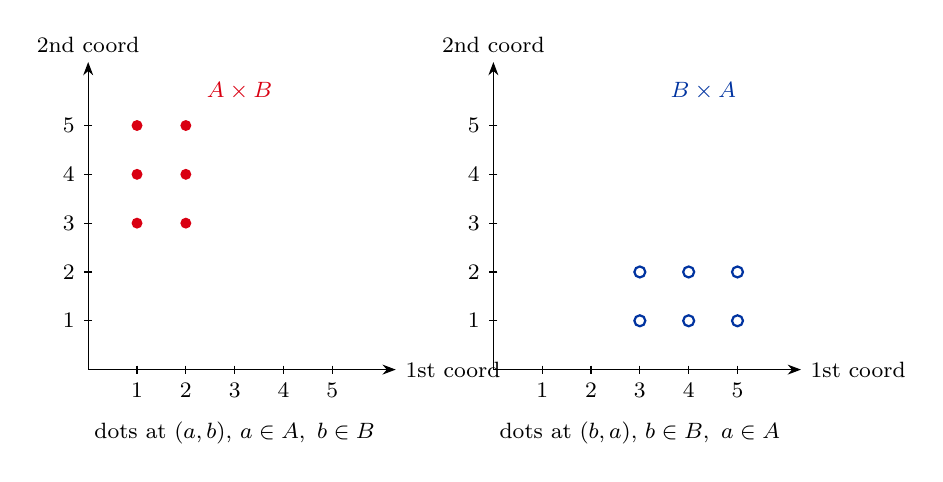
\begin{tikzpicture}[font=\footnotesize, scale=0.62, >=Stealth]
% ---- left: A x B  (x in A={1,2}, y in B={3,4,5}) ----
\begin{scope}
  \draw[->] (0,0) -- (6.3,0) node[right] {1st coord};
  \draw[->] (0,0) -- (0,6.3) node[above] {2nd coord};
  \foreach \x in {1,2,3,4,5}{\draw (\x,0.08)--(\x,-0.08) node[below]{$\x$};}
  \foreach \y in {1,2,3,4,5}{\draw (0.08,\y)--(-0.08,\y) node[left]{$\y$};}
  % A x B : a in {1,2}, b in {3,4,5}
  \foreach \a in {1,2}\foreach \b in {3,4,5}{\fill[armRed] (\a,\b) circle (3.2pt);}
  \node[armRed] at (3.1,5.7) {$A\times B$};
  \node at (3.0,-1.3) {dots at $(a,b)$, $a\in A,\ b\in B$};
\end{scope}
% ---- right: B x A  (x in B={3,4,5}, y in A={1,2}) ----
\begin{scope}[shift={(8.3,0)}]
  \draw[->] (0,0) -- (6.3,0) node[right] {1st coord};
  \draw[->] (0,0) -- (0,6.3) node[above] {2nd coord};
  \foreach \x in {1,2,3,4,5}{\draw (\x,0.08)--(\x,-0.08) node[below]{$\x$};}
  \foreach \y in {1,2,3,4,5}{\draw (0.08,\y)--(-0.08,\y) node[left]{$\y$};}
  % B x A : b in {3,4,5}, a in {1,2}
  \foreach \b in {3,4,5}\foreach \a in {1,2}{\draw[armBlue, thick, fill=white] (\b,\a) circle (3.2pt);}
  \node[armBlue] at (4.3,5.7) {$B\times A$};
  \node at (3.0,-1.3) {dots at $(b,a)$, $b\in B,\ a\in A$};
\end{scope}
\end{tikzpicture}
\end{center}
The red and blue point sets are reflections across the diagonal; they overlap only on the diagonal,
so $A\times B=B\times A$ can hold only when $A=B$.

\answer{For nonempty $A,B$: $A\times B=B\times A\Rightarrow A=B$, proved by the two inclusions.
The nonemptiness is needed: $A=\varnothing$, $B=\{1\}$ is a counterexample without it.}

\begin{methodbox}
\textbf{Transferable technique:} to prove a set equality $A=B$, prove $A\subseteq B$ and
$B\subseteq A$ separately (\textquotedbl{}take an arbitrary element, show it lies in the
other\textquotedbl{}). When products appear, read off the coordinate that carries the information:
the first coordinate of a pair in $X\times Y$ lives in $X$, the second in $Y$. And always test an
\textquotedbl{}obvious\textquotedbl{} implication on the empty set before trusting it.
\end{methodbox}

% ============================================================================
% PROBLEM 60
% ============================================================================
\section*{Problem 60 - Cartesian-product distributive laws}

\begin{problembox}[60]
Prove the identities (1)--(6):
\begin{enumerate}[label=\textbf{(\arabic*)},leftmargin=1.4cm,itemsep=1pt]
\item $A\times(B\cup C)=(A\times B)\cup(A\times C)$;
\item $(B\cup C)\times A=(B\times A)\cup(C\times A)$;
\item $A\times(B\cap C)=(A\times B)\cap(A\times C)$;
\item $(B\cap C)\times A=(B\times A)\cap(C\times A)$;
\item $A\times(B\setminus C)=(A\times B)\setminus(A\times C)$;
\item $(B\setminus C)\times A=(B\times A)\setminus(C\times A)$.
\end{enumerate}
\end{problembox}

\begin{ideabox}
Every element of a product is an ordered pair $(x,y)$, and \textquotedbl{}$(x,y)\in
X\times Y$\textquotedbl{} is just the conjunction \textquotedbl{}$x\in X$ \emph{and} $y\in
Y$\textquotedbl{}. So the moment you write $(x,y)$ and unfold both sides into statements about
$x$ and $y$ separately, each identity becomes a tiny piece of propositional logic: $\cup$ is
\textquotedbl{}or\textquotedbl{} on the $y$-part, $\cap$ is \textquotedbl{}and\textquotedbl{},
$\setminus$ is \textquotedbl{}and not\textquotedbl{}, and the fixed factor $x\in A$ just rides
along unchanged. Prove (1), (3), (5) by this ordered-pair iff method; (2), (4), (6) are the
\emph{same} proofs with the product on the other side - swap the roles of the coordinates.
\end{ideabox}

\textbf{(1) Union on the right factor.}
\begin{align*}
(x,y)\in A\times(B\cup C)
&\iff x\in A\ \text{and}\ (y\in B\ \text{or}\ y\in C)\\
&\iff (x\in A\ \text{and}\ y\in B)\ \text{or}\ (x\in A\ \text{and}\ y\in C)
   &&\text{[distribute \textquotedbl{}and\textquotedbl{} over \textquotedbl{}or\textquotedbl{}]}\\
&\iff (x,y)\in A\times B\ \text{or}\ (x,y)\in A\times C\\
&\iff (x,y)\in(A\times B)\cup(A\times C). \qquad\blacksquare
\end{align*}

\textbf{(3) Intersection on the right factor.} Same chase with \textquotedbl{}and\textquotedbl{}:
\begin{align*}
(x,y)\in A\times(B\cap C)
&\iff x\in A\ \text{and}\ y\in B\ \text{and}\ y\in C\\
&\iff (x\in A\ \text{and}\ y\in B)\ \text{and}\ (x\in A\ \text{and}\ y\in C)
   &&\text{[$x\in A$ duplicated freely]}\\
&\iff (x,y)\in(A\times B)\cap(A\times C). \qquad\blacksquare
\end{align*}

\textbf{(5) Difference on the right factor.}
\begin{align*}
(x,y)\in A\times(B\setminus C)
&\iff x\in A\ \text{and}\ y\in B\ \text{and}\ y\notin C.
\end{align*}
On the other side,
$$(x,y)\in(A\times B)\setminus(A\times C)\iff (x\in A\ \text{and}\ y\in B)\ \text{and}\ \neg(x\in A\ \text{and}\ y\in C).$$
But the first clause already gives $x\in A$, so $\neg(x\in A\ \text{and}\ y\in C)$ collapses to
$y\notin C$. Hence this is $x\in A$ and $y\in B$ and $y\notin C$ - identical to the line above. So
the two sets are equal. $\blacksquare$

\textbf{(2), (4), (6) - the mirror images.}
These are (1), (3), (5) with the variable factor $A$ moved to the \emph{first} coordinate. Run the
identical argument on a pair $(y,x)$ with $(y,x)\in X\times A\iff y\in X$ and $x\in A$; the fixed
part is now $x\in A$ in the second slot, and $\cup,\cap,\setminus$ distribute over the $y$-part
exactly as before. Concretely:
\begin{align*}
(y,x)\in(B\cup C)\times A &\iff (y\in B\ \text{or}\ y\in C)\ \text{and}\ x\in A
  \iff (y,x)\in(B\times A)\cup(C\times A),\\
(y,x)\in(B\cap C)\times A &\iff y\in B\ \text{and}\ y\in C\ \text{and}\ x\in A
  \iff (y,x)\in(B\times A)\cap(C\times A),\\
(y,x)\in(B\setminus C)\times A &\iff y\in B\ \text{and}\ y\notin C\ \text{and}\ x\in A
  \iff (y,x)\in(B\times A)\setminus(C\times A).\qquad\blacksquare
\end{align*}

\textbf{Always check.} All six identities were verified by exhaustive enumeration over every triple
$A,B,C$ of subsets of $\{0,1,2\}$ (so every possible product was compared elementwise);
\emph{zero} mismatches. \checkmark

\textbf{The distributive law (1) as an area picture.} Draw $A$ as an interval on the $x$-axis and
$B$, $C$ as two stacked bands on the $y$-axis. A product $X\times Y$ is the rectangle \textquotedbl{}above
$X$, beside $Y$\textquotedbl{}. Then $A\times(B\cup C)$ is the full block over $A$ spanning $B$ and
$C$, which is exactly the $A\times B$ rectangle stacked on the $A\times C$ rectangle:

\begin{center}
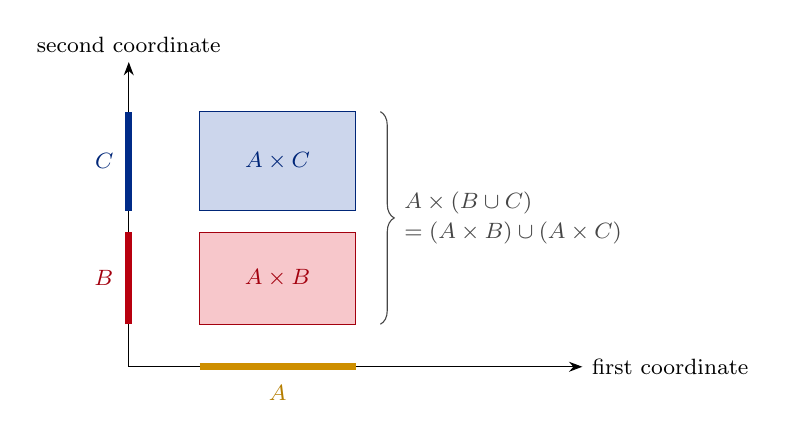
\begin{tikzpicture}[font=\footnotesize, scale=0.9, >=Stealth]
% axes
\draw[->] (0,0) -- (6.4,0) node[right] {first coordinate};
\draw[->] (0,0) -- (0,4.3) node[above] {second coordinate};
% A on x-axis : interval [1,3.2]
\draw[armOrange!85!black, line width=2.4pt] (1,0) -- (3.2,0);
\node[armOrange!75!black, anchor=north] at (2.1,-0.12) {$A$};
% B and C bands on y-axis
\draw[armRed!85!black, line width=2.4pt] (0,0.6) -- (0,1.9);
\node[armRed!75!black, anchor=east] at (-0.08,1.25) {$B$};
\draw[armBlue!85!black, line width=2.4pt] (0,2.2) -- (0,3.6);
\node[armBlue!75!black, anchor=east] at (-0.08,2.9) {$C$};
% A x B rectangle
\fill[armRed!22] (1,0.6) rectangle (3.2,1.9);
\draw[armRed!75!black] (1,0.6) rectangle (3.2,1.9);
\node[armRed!75!black] at (2.1,1.25) {$A\times B$};
% A x C rectangle
\fill[armBlue!20] (1,2.2) rectangle (3.2,3.6);
\draw[armBlue!75!black] (1,2.2) rectangle (3.2,3.6);
\node[armBlue!75!black] at (2.1,2.9) {$A\times C$};
% brace on right: union spans B u C
\draw[decorate, decoration={brace, amplitude=5pt}, gray!55!black] (3.55,3.6) -- (3.55,0.6);
\node[gray!55!black, anchor=west, align=left] at (3.75,2.1)
  {$A\times(B\cup C)$\\[1pt]$=(A\times B)\cup(A\times C)$};
\end{tikzpicture}
\end{center}

\answer{All six hold. The right-factor laws (1),(3),(5) follow from
$(x,y)\in X\times Y\iff x\in X\wedge y\in Y$, distributing the set operation over the
$y$-coordinate while $x\in A$ rides along; the left-factor laws (2),(4),(6) are the same with the
coordinates swapped.}

\begin{methodbox}
\textbf{Transferable technique:} a Cartesian product turns set algebra into logic on coordinates -
$(x,y)\in X\times Y\iff (x\in X)\wedge(y\in Y)$. To prove a product identity, write a generic pair
$(x,y)$, expand both sides into and/or/not statements about the two coordinates, and use ordinary
logical distribution. A constant factor (here $A$) simply appears, unchanged, in the same
coordinate on both sides.
\end{methodbox}

\end{document}
